\section{Mathematical preliminaries} \label{tex:math_prelim}

\cite{Church:1940:A-formulation-of-the-simple-theory-of-types}


In this section, based on~\cite{Barendregt:1981:The-Lambda-Calculus:-Its-Syntax-and-Semantics},~\cite{Barendregt:1992:Lambda-Calculi-with-Types} and~\cite{HindleySeldin:2008:Lambda-Calculus-and-Combinators-an-Introduction}, the basic definitions and theorems of type-free (\ref{sec:A1}) and simply-typed (\ref{sec:A2}) lambda calculus are presented. 

\subsection{Type-free Lambda Calculus} \label{sec:A1}

\begin{definition}[$\lambda$-terms] The set of \textbf{$\lambda$-terms} $\Lambda$ constructed from an enumerable set of variables $V = \{ v, v_1 ,v_2, \dots\}$ is defined inductively as follows:
\begin{center}
$
\begin{array}{rcll}
x \in V & \Longrightarrow & x \in \Lambda &\\
M,N \in \Lambda &  \Longrightarrow & (MN) \in \Lambda & \text{(\textbf{application})}\\ 
 x \in V, M \in \Lambda&  \Longrightarrow  & (\lambda x.M) \in \Lambda & \text{(\textbf{abstraction})}
\end{array} 
$
\end{center}
\end{definition}

In the term $ (\lambda x.M)$, called abstraction, the variable $x$ is the \textbf{argument} of the function and $M$ is the \textbf{body} of the function. %The variable $x$ is \textbf{bound} by $\lambda$ in  $ (\lambda x.M)$.

\begin{example} \label{app:ex1} The following are $\lambda$-terms:
\begin{align*}
& x \\
& (x_1x_2) \\
& (\lambda x. (x_1 x_2)) \\
& (\lambda x_1. (x_1 x_2)) \\
& ((\lambda x. (x_1 x_2)) x_3 ) 
\end{align*}
\end{example}


\begin{remark}[Parenthesis conventions] \label{rem:parcon}
\begin{itemize}
\item application is left-associative
$$MN_1 N_2 \dots N_n \seq (\dots ( (MN_1) N_2 ) \dots N_n)$$
\item  a sequence of $\lambda$-abstractions $\lambda x_1. (\lambda x_2. ( \dots (\lambda x_n. M) )  ) $ is abbreviated as \\ $\lambda x_1 x_2 \dots x_n.M$
$$\lambda x_1 x_2 \dots x_n.M \seq \lambda x_1. (\lambda x_2. ( \dots (\lambda x_n. M) )  )  $$
\item parentheses surrounding the body of an abstraction can be dropped
$$\lambda x_1 x_2 \dots x_n.(M) \seq \lambda x_1 x_2 \dots x_n.M$$
\item outermost parentheses can be dropped 
$$(M) \seq M$$
\end{itemize}
\end{remark}
%application has a higher precedence than abstraction. 
Note that according to the conventions on parentheses, term $\lambda x. MN$ is a more concise way of writing $\lambda x. (MN)$ and is not equivalent to $(\lambda x. M)N$. 

\begin{example} According to Remark~\ref{rem:parcon}, the $\lambda$-terms in Example~\ref{app:ex1} can be written as follows:
\begin{align*}
& x \\
& x_1x_2 \\
& \lambda x. x_1 x_2 \\
& \lambda x_1. x_1 x_2 \\
& (\lambda x. x_1 x_2) x_3 
\end{align*}
\end{example}



\begin{definition}[Free and bound variables] A variable $x$ is \textbf{free} in a $\lambda$-term $M$ if $x$ is not in the scope of $\lambda x$. If $x$ is in the scope of $\lambda x$, it is \textbf{bound}.
\end{definition}

\begin{example} In the term $ (\lambda x. x_1 x_2)$, the variables $x_1$ and $x_2$ are free. In the term $(\lambda x_1. x_1 x_2)$, the variable $x_1$ is bound and the variable $x_2$ is free. In the term $x(\lambda x.x)$, the variable occurs free in the subterm $x$ and bound in the subterm $\lambda x.x$. 
\end{example}

\begin{definition}[Closed $\lambda$-terms] \ 
\begin{enumerate}
\item The set of \textbf{free variables} of $M$, $FV(M)$ is defined inductively as follows:
\begin{align*}
 FV(x)  & = \{ x \} \\
 FV(\lambda x.M)  & = FV(M) - \{ x \} \\
 FV(MN)  & = FV(M) \cup FV(N)
\end{align*}
\item M is \textbf{closed} or a \textbf{combinator}, if $FV(M) = \emptyset$
%\item The result of \textbf{substitution} of $N$ for (the free occurrences of) $x$ in $M$, denoted $x[x:=N]$, is defined as follows ($x \neq y$):
%\begin{center}
%$
%\begin{array}{rcl}
%x[x:=N] & \defeq & N \\
%y[x:=N] &  \defeq & y\\ 
%(PQ)[x:=N]&  \defeq  & (P[x:=N])(Q[x:=N])\\
%(\lambda y.P)[x:=N] & \defeq & \lambda y.(P[x:=N]) \\
%(\lambda x.P)[x:=N] & \defeq & \lambda x.P
%\end{array} 
%$
%\end{center}
\end{enumerate}
\end{definition}

If an equation $M=N$ is provable in the lambda calculus, the provability is denoted by $\lambda \vdash M = N$
or sometimes just by $M=N$.

\begin{definition}[Axioms and rules] For all $M,N, L,Z \in \Lambda$ the following axioms and rules hold:
\begin{prooftree}
\AXC{} \RightLabel{$\beta$-conversion}
\UIC{$(\lambda x.M)N = M[x:=N]$}
\end{prooftree}

\begin{prooftree}
\AXC{}
\UIC{$M = M$}
\end{prooftree}

\begin{prooftree}
\AXC{$M = N$}
\UIC{$N = M$}
\end{prooftree}

\begin{prooftree}
\AXC{$M=N$}
\AXC{$N=L$}
\BIC{$M=L$}
\end{prooftree}

\begin{prooftree}
\AXC{$M=N$}
\UIC{$MZ=NZ$}
\end{prooftree}

\begin{prooftree}
\AXC{$M=N$}
\UIC{$ZM=ZN$}
\end{prooftree}

\begin{prooftree}
\AXC{$M=N$} \RightLabel{rule $\xi$}
\UIC{$\lambda x.M=\lambda x.N$}
\end{prooftree}

\end{definition}

Importantly, substitution $[x:=N]$ in $M$, denoted $M[x:=N]$, is only applicable to the free occurrences of $x$ in $M$. For example,
\begin{align*}
(xy(\lambda x.x))[x:=N] = Ny(\lambda x.x)
\end{align*}

\begin{definition}[Substitution] The result of \textbf{substitution} of $N$ for the free occurences of $x$ in $M$, i.e. $M[x:=N]$, is defined inductively on the structure of $M$ as follows:
\begin{align*}
 x[x:=N] \defeq  \ & N \\
 y[x:=N] \defeq  \ &  y \ \ \text{provided} \ x \nseq y \\
 (\lambda y.M_1)[x:=N] \defeq   \ & \lambda y. (M_1 [x:=N]) \\
 (M_1 M_2)[x:=N] \defeq  \  & (M_1[x:=N])(M_2[x:=N]) \\
 (\lambda x.M_1)[x:=N]  \defeq \ & \lambda x.M_1
\end{align*}

\end{definition}

\begin{lemma}[Substitution lemma] If  $x \nseq y$ and $x \notin FV(L)$, then
\begin{align*}
 M[x:=N][y:=L] \seq M[y:=L][x:=N[y:=L]]
\end{align*}
\end{lemma}
\begin{proof} The proof is by induction on the structure of $M$.
\end{proof}


When performing a substitution $M[x:=N]$, it is necessary to rename those bound variables in $M$ that are free in N. Otherwise, the substitution 
may lead to a false result. For example, without renaming the bound variable $x$ in $\lambda x.xy$, the substitution  $(\lambda x.xy)[y:=x]$ leads to the term $\lambda x.xx$ that acts differently from the desired term, because the free variable $x$ became bound. However, changing $x$ to $z$, for example, before making the substitution, leads to the desired term $\lambda z.zx$. 

\begin{definition}[$\alpha$-conversion] A \textbf{change of bound variable} $x$ in $M$, or an \textbf{$\alpha$-conversion} in $M$, is the replacement of an occurrence of $\lambda x.N$ in $M$ by $\lambda y.(N[x:=y])$, where $y$ does not occur in $N$.
\end{definition}

\begin{definition}[$\alpha$-congruency] $M$ and $N$ are \textbf{$\alpha$-congruent}, denoted $M \congr N$, if one can result from the other by a finite series of changes of bound variables.
\end{definition}

\begin{example}
\begin{align*}
& \lambda x.xy \congr \lambda z.zy \ncongr \lambda x.xx \\
& \lambda xy.yx(\lambda x.x) \congr \lambda xy. yx(\lambda z.z)  \congr \lambda zy. yz(\lambda x.x) \\
& \lambda xy.yx\congr  \lambda zy. yz \congr  \lambda zx. xz \congr \lambda yx. xy 
\end{align*}
\end{example}

It is natural to identify the terms that are $\alpha$-congruent, as they represent the same processes. Moreover, the same processes can be represented by different terms. For example, $\lambda x.Mx$ and $M$ both lead to $MN$ when applied to $N$. Hence, the following rule can be introduced:
\begin{definition}[Extensionality] \textbf{Extensionality} is the following derivation rule, provided $x \notin FV(MN)$:
\begin{prooftree}
\AXC{$Mx = Nx$}
\UIC{$M = N$}
\end{prooftree}
\end{definition}
The extensionality rule allows to prove $\lambda x. Mx = M$. Alternatively,  $\lambda x. Mx = M$ can be considered to be an axiom:
\begin{definition}[$\eta$-conversion] Let $x \notin FV(M)$. Then
\begin{prooftree}
\AXC{} \RightLabel{$\eta$-conversion}
\UIC{$\lambda x. Mx = M$}
\end{prooftree}
\end{definition}

\begin{definition}[$\beta$-normal form]
\begin{enumerate}
\item $M$ is a \textbf{$\beta$-normal form}, if $M$ has no subterm of the form $(\lambda x.L)K$
\item $M$ \textbf{has a $\beta$-normal form}, if there exists an $N$ such that $N$ is a $\beta$-normal form and $N = M$.
\end{enumerate}
\end{definition}

When $M$ is a $\beta$-normal form, it is often said that $M$ is in normal form.

\begin{example} \
\begin{enumerate}
\item $\lambda x.x$ is in normal form.
\item $(\lambda x.x)y$ has a normal form, namely $y$.
\item $(\lambda xy.y)z$ has a normal form, namely $(\lambda y.y)$.
\item $(\lambda xy.x)z$ has a normal form, namely $z$.
\item $(\lambda x.xx)(\lambda y.yy)$ has no normal form.
\end{enumerate}
\end{example}

A notion of reduction on $\Lambda$ is a binary relation on $\Lambda$. The classical notion of reduction $\beta$ is defined as follows:
\begin{definition} $\beta = \{ ( (\lambda x. M)N , M[x:=N] ) | M, N \in \Lambda  \} $
\end{definition}

\begin{definition}[$\beta$-redex, $\beta$-contractum] 
A \textbf{$\beta$-redex} is a term $M$ such that $(M,N) \in \beta$ for some term $N$. In this case $N$ is called \textbf{$\beta$-contractum} of $M$.
\end{definition}

\begin{definition} The notion of reduction $\beta$ induces the following binary relations:
\begin{align*}
\bconv \  & \textbf{one-step } \beta \textbf{-reduction} \\
\bred \  &  \beta \textbf{-reduction} \\
=_{\beta} \  & \beta \textbf{-equality} \text{ (also called } \beta \textbf{-convertibility}\text{)} 
\end{align*}
These relations are inductively defined as follows:
\begin{center}
$
\begin{array}{rcl}
(M,N) \in \beta & \Longrightarrow & M \bconv N \\
M \bconv N &  \Longrightarrow & ZM \bconv ZN \\ 
M \bconv N &  \Longrightarrow & MZ \bconv NZ \\ 
M \bconv N & \Longrightarrow & \lambda x.M \bconv \lambda x.N \\
& & \\
M \bconv N &  \Longrightarrow & M \bred N \\ 
M \bred M & \\ 
M \bred N, N \bred Z & \Longrightarrow & M \bred Z \\
&& \\
M \bred N &  \Longrightarrow & M =_{\beta} N \\ 
M =_{\beta} N & \Longrightarrow & N =_{\beta} M\\ 
M =_{\beta} N, N =_{\beta} Z & \Longrightarrow & M =_{\beta} Z 
\end{array} 
$
\end{center}


%\begin{enumerate}
%\item $(M,N) \in \beta$
%\end{enumerate}

\end{definition}

The notions of $\beta$-redex and $\beta$-equality allow to give an alternative, more formal, definition of $\beta$-normal form:
\begin{definition}[$\beta$-normal form]  
\begin{enumerate}
\item A term $N$ is called a $\beta$-normal form, if $N$ does not contain (as subterm) any $\beta$-redex.
\item A term $N$ is a $\beta$-normal form of $M$, if $N$ is a $\beta$-normal form and $M =_{\beta} N$.
\end{enumerate}
\end{definition}

%\begin{definition}[$\beta$-contractum, $\beta$-redex] Any term of the form 
%\begin{align*} (\lambda x.M)N
%\end{align*}
%is called a \textbf{$\beta$-redex} and the corresponding term
%\begin{align*} M[x:=N]
%\end{align*}
%is called its \textbf{contractum}.
%\end{definition}

%
%\begin{definition}[$\beta$-contracting, $\beta$-reducing]ff
%\end{definition}

The notion of $\beta$-reduction is very important, because it characterizes provability in $\lambda$ and it is Church-Rosser:

\begin{proposition} $M =_{\beta} N$ iff $\lambda \vdash M = N$
\end{proposition}
\begin{proof} See~\cite[p.59]{Barendregt:1981:The-Lambda-Calculus:-Its-Syntax-and-Semantics}.
%\begin{itemize}
%\item Assume $\lambda \vdash M = N$. Use the induction on the length of the proof of $M=N$.
%\item Assume $M =_{\beta} N$. Show by induction on the definition of the relations involved that
%\end{itemize}
\end{proof}


\begin{theorem}[Church-Rosser theorem for $\bred$] If $L \bred M$ and $L \bred N$, then there exists a term $Z$ such that $M \bred Z$ and $N \bred Z$.
\end{theorem}
\begin{proof} See~\cite[p.62]{Barendregt:1981:The-Lambda-Calculus:-Its-Syntax-and-Semantics} or~\cite[p.289]{HindleySeldin:2008:Lambda-Calculus-and-Combinators-an-Introduction}.
\end{proof}
\begin{figure}[h!]
  \centering
    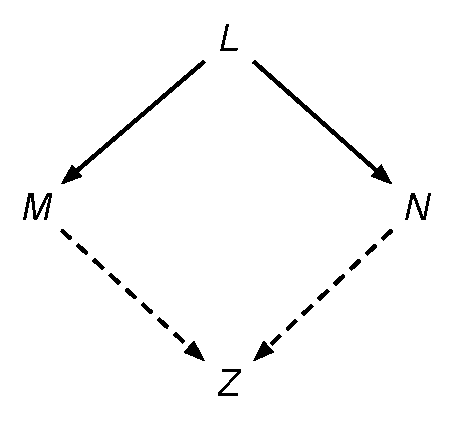
\includegraphics[width=0.3\textwidth]{images/Diamond.pdf}
      \caption{Diamond property.} \label{fig:diamond}
\end{figure}

The Church-Rosser theorem says that for two $\beta$-convertible terms, there is a term to which they both $\beta$-reduce, as illustrated in Figure~\ref{fig:diamond}. The property described in the theorem, that if a term can be reduced to two different terms, then these two terms can be further reduced to one term, is called the \textbf{diamond property} or \textbf{confluence}. The theorem states that $\beta$-reduction is confluent.

\subsection{Simply-typed Lambda Calculus}  \label{sec:A2}

Lambda terms can be assigned expressions, called ``types'', to denote their intended input and output sets. There exists two typing paradigms: 
\`{a} la Curry, sometimes called \textbf{implicit}, and \`{a} la Church, sometimes called \textbf{explicit}. This section first recalls the basics of Curry-style approach and then briefly compares it with the Church-style.

\begin{definition}[Simple types] Given a set $A$ of \textbf{atomic types}, the set of \textbf{types} $T$ is inductively defined as follows:
\begin{center}
$
\begin{array}{rcll}
\alpha \in A & \Longrightarrow & \alpha \in T &\\
\alpha, \beta \in A &  \Longrightarrow & (\alpha \rightarrow \beta) \in T & \text{(\textbf{function types})}
\end{array} 
$
\end{center}
\end{definition}
An atomic type is intended to denote some particular set. A function type $(\alpha \rightarrow \beta)$ is intended to denote some set of functions from $\alpha$ to $\beta$, i.e. the functions that take as the argument a member of the set denoted by $\alpha$ and return as an output a member of the set denoted by $\beta$.


\begin{remark}[Parenthesis convention] A complex functional type $(\alpha_1 \rightarrow (\alpha_2 \rightarrow \dots \rightarrow (\alpha_{n-1} \rightarrow \alpha_n)  \dots ))$ is abbreviated as $\alpha_1 \rightarrow \alpha_2 \rightarrow \dots \rightarrow \alpha_n$ (i.e. parentheses are associated to the right):
\begin{align*}
(\alpha_1 \rightarrow (\alpha_2 \rightarrow \dots \rightarrow (\alpha_{n-1} \rightarrow \alpha_n)  \dots )) & \seq \alpha_1 \rightarrow \alpha_2 \rightarrow \dots \rightarrow \alpha_n
\end{align*}
\end{remark}


\begin{definition}[$\lambda\!\rightarrow$-Curry]
\begin{enumerate}
\item A \textbf{statement} is of the form $M:\sigma$ with $M \in \Lambda$ and $\sigma \in T$. The type $\sigma$ is the \textbf{predicate} and the term $M$ is the \textbf{subject} of the statement.
\item A \textbf{declaration} is a statement with a variable as a subject.
\item A \textbf{basis} is a set of declarations with distinct variables as subjects.
\end{enumerate}
\end{definition}


\begin{definition}[Derivation rules in $\lambda\!\rightarrow$-Curry] A statement $M:\sigma$ is \textbf{derivable} from a basis $\Gamma$, denoted $\Gamma \vdash_{\lambda\rightarrow \text{-Curry}} M: \sigma$ , $\Gamma \vdash_{\lambda\rightarrow} M: \sigma$ or simply $\Gamma \vdash M: \sigma$, if $\Gamma \vdash M: \sigma$ can be produced by the following rules:
 
\begin{prooftree}
\AXC{} \RightLabel{axiom}
\UIC{$\Gamma, x: \alpha \vdash x: \alpha $}
\end{prooftree} 
 
 \begin{prooftree}
\AXC{$\Gamma \vdash M: \alpha \rightarrow \beta$}
\AXC{$\Gamma \vdash N: \alpha$} \RightLabel{app}
\BIC{$\Gamma \vdash MN: \beta$}
\end{prooftree}

\begin{prooftree}
\AXC{$\Gamma, x: \alpha \vdash M:\beta$} \RightLabel{abs}
\UIC{$\Gamma \vdash \lambda x.M: \alpha \rightarrow \beta$}
\end{prooftree}

\end{definition}


%\begin{definition}
%
%\medskip \noindent \textbf{Compatibility rules}:
%
%\begin{prooftree}
%\AXC{} \RightLabel{if $x$ is a variable}
%\UIC{$x \evalto x$}
%\end{prooftree}
%
%\begin{prooftree}
%\AXC{} \RightLabel{if $c$ is a constant}
%\UIC{$c \evalto c$}
%\end{prooftree}
%
%\begin{prooftree}
%\AXC{$M \evalto N$}
%\UIC{$\lambda x. M \evalto \lambda x.N $}
%\end{prooftree}
%
%\begin{prooftree}
%\AXC{$M \evalto \lambda x. K$}
%\AXC{$Q \evalto N$}
%\AXC{$K[x:=N] \evalto O$}
%\TIC{$ MQ \evalto O$}
%\end{prooftree}
%
%\begin{prooftree}
%\AXC{$M \evalto x$}
%\AXC{$Q \evalto N$}
%\BIC{$ MQ \evalto xN$}
%\end{prooftree}
%
%\begin{prooftree}
%\AXC{$M \evalto OK$}
%\AXC{$Q \evalto N$}
%\BIC{$ MQ \evalto OKN$}
%\end{prooftree}
%\end{definition}

\begin{lemma}[Substitution lemma for $\lambda\!\rightarrow$-Curry] \label{lem:substitution-Curry} \
\begin{enumerate}
\item If $\Gamma \vdash M:\sigma$, then $\Gamma[\alpha :=\tau] \vdash M:\sigma[\alpha :=\tau]$.
\item Suppose $\Gamma, x: \sigma \vdash M: \tau$ and $\Gamma \vdash N: \sigma$. Then $\Gamma \vdash M[x:=N]: \tau$.
\end{enumerate}
\end{lemma}
\begin{proof} 
\begin{enumerate}
\item The proof is by induction on the derivation of $M:\sigma$.
\item The proof is by induction on the generation of $\Gamma, x: \sigma \vdash M:\tau$
\end{enumerate}
\end{proof}

The following theorem states that the set of terms having a certain type is closed under reduction:
\begin{theorem}[Subject reduction theorem for $\lambda\!\rightarrow$-Curry] Suppose $M \bred N$. Then 
\begin{center}
$
\begin{array}{rcl}
\Gamma \vdash M: \sigma &\Longrightarrow & \Gamma \vdash N: \sigma
\end{array}
$
\end{center}
\end{theorem}
\begin{proof} See~\cite[p.41]{Barendregt:1992:Lambda-Calculi-with-Types}.
\end{proof}

While in Curry's approach each term is assigned a type after the term has been built, in Church's approach, the type of a term is integrated in the term itself. For example, the term $\lambda x.x$ can be assigned a type according to the Curry and Church styles respectively as follows:
\begin{align*}
& \vdash_{Curry} \lambda x.x: (\sigma \rightarrow \sigma) \\
& \vdash_{Church} \lambda x^\sigma.x: (\sigma \rightarrow \sigma) 
\end{align*}
The term $\lambda x^\sigma.x$ itself is annotated in a Church system by $\sigma$. This means that $\lambda x^\sigma.x$ takes the argument $x$ from the particular set denoted by $\sigma$. In contrast, a Curry system allows each term to have a polymorphic type. For example, the term $\lambda x.x:  (\sigma \rightarrow \sigma)$ denotes the operation of doing nothing regardless how $\sigma$ is instantiated: it can stand, for example, for integers or for booleans. 

\begin{definition}[$T$-annotated $\lambda$-terms] Let $V$ be a set of variables, $T$ be a set of types. The set $\Lambda_T$ of $T$\textbf{-annotated} $\lambda$\textbf{-terms} is defined as follows:
\begin{center}
$
\begin{array}{rcl}
x \in V & \Longrightarrow & x \in \Lambda_T \\
M, N \in  \Lambda_T& \Longrightarrow & MN \in \Lambda_T \\
x \in V, M \in \Lambda_T, \sigma \in T & \Longrightarrow & \lambda x^\sigma.M \in \Lambda_T
\end{array}
$
\end{center}
\end{definition}

The typed lambda calculus  \`{a} la Church is defined similarly to the typed lambda calculus  \`{a} la Curry: an important difference is in the derivation rule corresponding to the abstraction: the abstracted variable is explicitly annotated with a type in the Church-style system.
The explicit annotation of types in Church-style system makes it possible to decide whether a term has a certain type. This is an undecidable question for some Curry systems. On the other hand, a Curry-style system has more power and more flexibility than a Church-style system. For example, the easiest way to answer the question whether an untyped term $M$ has any typed analogues is to re-state the question in Curry's notation. Furthermore, Curry-style systems can be generalized in ways Church-style systems cannot. 

Terms \`{a} la Church can be easily mapped into terms \`{a} la Curry. This is done simply by ``erasing'' all type annotations within the term \`{a} la Church:
\begin{definition} $| \cdot |: \Lambda_T \rightarrow \Lambda$ is defined as follows:
\begin{center}
$
\begin{array}{rcl}
|x|& \defeq & x \\
|MN|& \defeq & |M||N| \\
|\lambda x^{\sigma}.M|& \defeq & \lambda x.|M|
\end{array}
$
\end{center}
\end{definition}
The following proposition states that terms in the Church version project to terms in the Curry version of $\lambda\!\rightarrow$; and that terms in the Curry style can be ``lifted'' to terms in the Church style:
\begin{proposition}  
\ 
\begin{enumerate}
\item Let $M \in \Lambda_T$. Then
\begin{align*}
\Gamma \vdash_{Church} M:\sigma  \ \ \Longrightarrow \ \ & \Gamma \vdash_{Curry} |M|:\sigma
\end{align*}
\item Let $N\in \Lambda$. Then
\begin{align*}
\Gamma \vdash_{Curry} N:\sigma  \ \  \Longrightarrow \ \ & \text{exists } M  \in \Lambda_T  \\
& \text{such that }  \Gamma \vdash_{Church}  M:\sigma \text{ and } |M| \congr N
\end{align*}
\end{enumerate}
\end{proposition}
\begin{proof} Both (1) and (2) are proved by induction on the given derivation.
\end{proof}
See~\cite{Barendregt:1992:Lambda-Calculi-with-Types}  and~\cite{HindleySeldin:2008:Lambda-Calculus-and-Combinators-an-Introduction} for profound introductions to the two typing styles and their detailed comparisons.